\documentclass[aspectratio=169,11pt]{beamer}
\usepackage{teaching_slides}
\usetikzlibrary{positioning,calc}

\title[Causal Diagrams]{ Econometrics I}
\subtitle{Lecture 5b: Causal Diagrams (DAGs)}
\author{Chris Conlon \\NYU Stern}
\date{Fall 2026}

% New deck (Fall 2026). Sources: Cunningham Mixtape Ch. 3;
% Hunermund & Bareinboim (2021); Cinelli, Forney & Pearl (2022),
% "A Crash Course in Good and Bad Controls".

\begin{document}
\maketitle


\begin{frame}{Two languages for the same problem}
\begin{itemize}
	\item \alert{Potential outcomes} (last hour) tell us \emph{what we want}:
	$\E[Y_i(1) - Y_i(0)]$, and what randomization buys us.

	\medskip
	\item \alert{Causal diagrams} (DAGs) encode \emph{what we believe}: which variables
	cause which, drawn as arrows. The assumptions are the \emph{missing} arrows.

	\medskip
	\item Why learn both?
	\begin{itemize}
		\item DAGs make ``what should I control for?'' a mechanical question with a
		right answer --- and expose when a control makes things \alert{worse}.
		\item Potential outcomes handle heterogeneity and identification-by-design
		more gracefully. Economists mostly publish in this language.
	\end{itemize}

	\medskip
	\item Readings: Mixtape Ch.~3; H\"unermund \& Bareinboim (2021); Cinelli, Forney \&
	Pearl (2022), ``A Crash Course in Good and Bad Controls.''
\end{itemize}
\end{frame}


\begin{frame}{What is a DAG?}
\begin{columns}
\begin{column}{0.45\textwidth}
\begin{center}
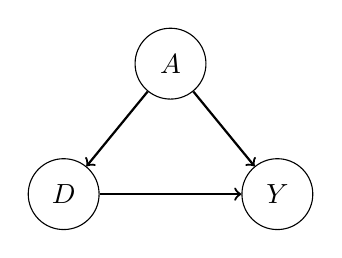
\begin{tikzpicture}[every node/.style={draw, circle, minimum size=9mm, inner sep=1pt}, node distance=18mm]
	\node (D) {$D$};
	\node[right=of D] (Y) {$Y$};
	\node[above=12mm of $(D)!0.5!(Y)$] (A) {$A$};
	\draw[->, thick] (D) -- (Y);
	\draw[->, thick] (A) -- (D);
	\draw[->, thick] (A) -- (Y);
\end{tikzpicture}
\end{center}
\smallskip
{\small $D$ = education, $Y$ = wages, $A$ = ability}
\end{column}
\begin{column}{0.55\textwidth}
\begin{itemize}
	\item Nodes are variables; arrows are direct causal effects; no cycles allowed
	(``acyclic'').

	\item Every \alert{missing arrow is an assumption}: this graph asserts nothing
	else causes both $D$ and $Y$.

	\item Unobserved variables (like ability) still belong in the graph --- being
	unobservable doesn't stop something from causing things.
\end{itemize}
\end{column}
\end{columns}
\end{frame}


\begin{frame}{Paths: how association travels}
In the graph on the last slide there are two paths from $D$ to $Y$:
\begin{enumerate}
	\item $D \rightarrow Y$: the \alert{causal path}. This is the thing we want to measure.
	\item $D \leftarrow A \rightarrow Y$: a \alert{backdoor path}. Association flows
	along it even though $D$ causes none of it.
\end{enumerate}
\bigskip
\begin{itemize}
	\item The regression of $Y$ on $D$ alone picks up \emph{both} paths --- this is
	exactly the omitted variables bias formula from Lecture 2, drawn as a picture.

	\medskip
	\item \alert{Identification strategy = a plan for shutting every backdoor path
	while leaving the causal path alone.}
\end{itemize}
\end{frame}


\begin{frame}{Good controls: closing a backdoor}
\begin{columns}
\begin{column}{0.45\textwidth}
\begin{center}
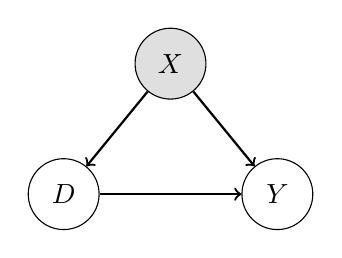
\begin{tikzpicture}[every node/.style={draw, circle, minimum size=9mm, inner sep=1pt}, node distance=18mm]
	\node (D) {$D$};
	\node[right=of D] (Y) {$Y$};
	\node[above=12mm of $(D)!0.5!(Y)$, fill=gray!25] (X) {$X$};
	\draw[->, thick] (D) -- (Y);
	\draw[->, thick] (X) -- (D);
	\draw[->, thick] (X) -- (Y);
\end{tikzpicture}
\end{center}
\smallskip
{\small Shading $=$ conditioned on.}
\end{column}
\begin{column}{0.55\textwidth}
\begin{itemize}
	\item Conditioning on a \alert{confounder} $X$ (regression control, matching,
	stratification) \alert{blocks} the backdoor path $D \leftarrow X \rightarrow Y$.

	\item This is the \alert{backdoor criterion} (informally): find a set of observed
	variables that blocks every backdoor path, condition on them, and the remaining
	association is causal.

	\item ``Selection on observables'' (matching, next month) is exactly the claim
	that such a set exists \emph{and you have it}.
\end{itemize}
\end{column}
\end{columns}
\end{frame}


\begin{frame}{Colliders: conditioning can \emph{open} a path}
\begin{columns}
\begin{column}{0.45\textwidth}
\begin{center}
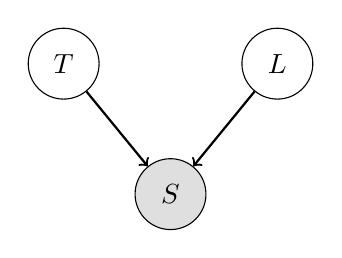
\begin{tikzpicture}[every node/.style={draw, circle, minimum size=9mm, inner sep=1pt}, node distance=18mm]
	\node (D) {$T$};
	\node[right=of D] (Y) {$L$};
	\node[below=12mm of $(D)!0.5!(Y)$, fill=gray!25] (C) {$S$};
	\draw[->, thick] (D) -- (C);
	\draw[->, thick] (Y) -- (C);
\end{tikzpicture}
\end{center}
\smallskip
{\small $T$ = talent, $L$ = luck, $S$ = startup gets funded.}
\end{column}
\begin{column}{0.55\textwidth}
\begin{itemize}
	\item $S$ is a \alert{collider} on the path $T \rightarrow S \leftarrow L$: two
	arrows collide into it. A collider \alert{blocks} the path \emph{by default}.

	\item But \alert{conditioning on a collider opens the path}: among \emph{funded}
	startups, talent and luck are negatively correlated --- if a funded founder wasn't
	talented, they must have been lucky.

	\item Talent and luck are independent in the population. The correlation is
	manufactured by the conditioning. This is \alert{selection bias, drawn as a picture}.
\end{itemize}
\end{column}
\end{columns}
\end{frame}


\begin{frame}{Bad control \#1: the post-treatment variable}
\begin{columns}
\begin{column}{0.45\textwidth}
\begin{center}
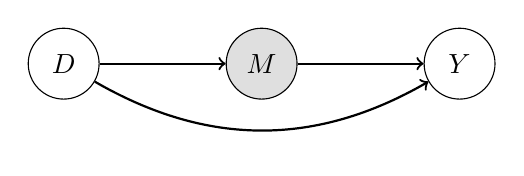
\begin{tikzpicture}[every node/.style={draw, circle, minimum size=9mm, inner sep=1pt}, node distance=16mm]
	\node (D) {$D$};
	\node[right=of D, fill=gray!25] (M) {$M$};
	\node[right=of M] (Y) {$Y$};
	\draw[->, thick] (D) -- (M);
	\draw[->, thick] (M) -- (Y);
	\draw[->, thick] (D) to[bend right=30] (Y);
\end{tikzpicture}
\end{center}
\smallskip
{\small $D$ = education, $M$ = occupation, $Y$ = wages}
\end{column}
\begin{column}{0.55\textwidth}
\begin{itemize}
	\item $M$ is a \alert{mediator}: part of \emph{how} education raises wages is by
	changing occupations.

	\item Controlling for occupation \alert{blocks part of the effect you are trying
	to measure}. The coefficient on $D$ is no longer the total effect.

	\item Rule of thumb with real teeth: \alert{do not control for variables that are
	themselves outcomes of the treatment}. When in doubt, ask: was this variable
	determined before or after $D$?
\end{itemize}
\end{column}
\end{columns}
\end{frame}


\begin{frame}{Bad control \#2: the collider / sample-selection control}
\begin{columns}
\begin{column}{0.45\textwidth}
\begin{center}
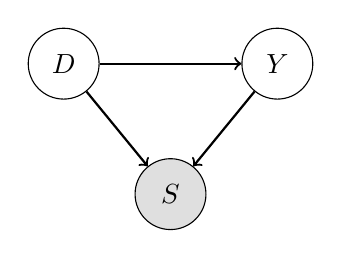
\begin{tikzpicture}[every node/.style={draw, circle, minimum size=9mm, inner sep=1pt}, node distance=16mm]
	\node (D) {$D$};
	\node[right=18mm of D] (Y) {$Y$};
	\node[below=12mm of $(D)!0.5!(Y)$, fill=gray!25] (S) {$S$};
	\draw[->, thick] (D) -- (Y);
	\draw[->, thick] (D) -- (S);
	\draw[->, thick] (Y) -- (S);
\end{tikzpicture}
\end{center}
\smallskip
{\small $D$ = ad exposure, $Y$ = purchase intent, $S$ = visits the site}
\end{column}
\begin{column}{0.55\textwidth}
\begin{itemize}
	\item Estimating the ad effect \alert{only among site visitors} conditions on a
	collider: both seeing the ad and wanting the product cause visits.

	\item Within visitors, exposure and intent are spuriously related even if the ad
	does nothing.

	\item This is the same disease as Heckman's sample selection (Lecture 11) and the
	``conditioning on graduation'' problem in education studies. \alert{Who is in your
	sample, and did the treatment help put them there?}
\end{itemize}
\end{column}
\end{columns}
\end{frame}


\begin{frame}{The research designs of this course, as DAGs}
\begin{columns}
\begin{column}{0.5\textwidth}
\begin{center}
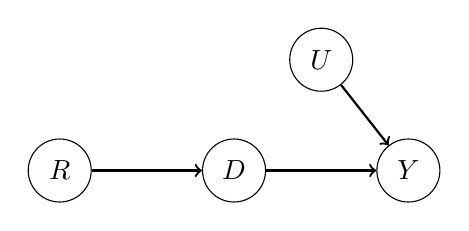
\begin{tikzpicture}[every node/.style={draw, circle, minimum size=8mm, inner sep=1pt}, node distance=14mm]
	\node (R) {$R$};
	\node[right=of R] (D) {$D$};
	\node[right=of D] (Y) {$Y$};
	\node[above=10mm of $(D)!0.5!(Y)$] (U) {$U$};
	\draw[->, thick] (R) -- (D);
	\draw[->, thick] (D) -- (Y);
	\draw[->, thick] (U) -- (Y);
\end{tikzpicture}\\
{\small \alert{Randomization}: coin flip $R$ causes $D$; no arrow into $D$ from $U$.}
\end{center}
\end{column}
\begin{column}{0.5\textwidth}
\begin{center}
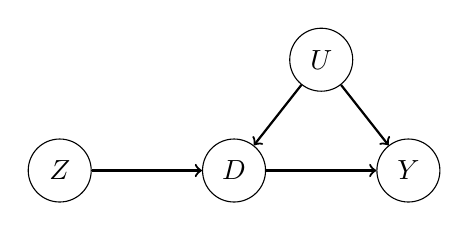
\begin{tikzpicture}[every node/.style={draw, circle, minimum size=8mm, inner sep=1pt}, node distance=14mm]
	\node (Z) {$Z$};
	\node[right=of Z] (D) {$D$};
	\node[right=of D] (Y) {$Y$};
	\node[above=10mm of $(D)!0.5!(Y)$] (U) {$U$};
	\draw[->, thick] (Z) -- (D);
	\draw[->, thick] (D) -- (Y);
	\draw[->, thick] (U) -- (D);
	\draw[->, thick] (U) -- (Y);
\end{tikzpicture}\\
{\small \alert{Instrumental variables}: the missing arrows $Z \rightarrow Y$ (exclusion)
and $U \rightarrow Z$ (exogeneity) ARE the IV assumptions.}
\end{center}
\end{column}
\end{columns}
\bigskip
Every design we meet from here on is a claim about missing arrows. When you referee a
paper, \alert{draw its DAG} --- the contestable assumption is usually an arrow the
authors need to be absent.
\end{frame}


\begin{frame}{Where DAGs strain (and economists push back)}
\begin{itemize}
	\item \alert{Simultaneity}: supply and demand determine price and quantity
	\emph{jointly} --- a cycle, which a DAG cannot draw. Our oldest identification
	problem (Working 1927, Lecture 6) sits awkwardly in this language.

	\medskip
	\item \alert{Heterogeneous effects}: LATE, compliers, and monotonicity
	(Lecture 7) are natural in potential outcomes and clumsy in DAGs.

	\medskip
	\item \alert{Where DAGs shine}: bad controls, sample selection, and transparent
	communication of assumptions --- especially in fields (marketing, IS) where
	``we controlled for everything'' is still treated as a virtue.

	\medskip
	\item Verdict: use the DAG to decide \emph{what to control for}; use potential
	outcomes to decide \emph{what your estimate means}.
\end{itemize}
\end{frame}


\begin{frame}{Coming attraction: when units interfere}
\begin{itemize}
	\item Everything today assumed my treatment doesn't affect \emph{your} outcome
	(part of \alert{SUTVA}). Drawn as a DAG: no arrows \emph{between units}.

	\medskip
	\item In marketplaces and platforms this fails constantly:
	\begin{itemize}
		\item Discounting rides for treated riders lengthens wait times for control riders.
		\item Promoting treated sellers steals demand from control sellers
		$\Rightarrow$ the A/B test \alert{overstates} the effect of the promotion.
	\end{itemize}

	\medskip
	\item Fixes people use: cluster-randomize markets, switchback designs,
	exposure modeling. See Wager Chs.~11--12 --- and Econometrics~II if you want the
	full treatment.

	\medskip
	\item For now: when someone shows you an experiment on a \alert{connected} system,
	ask what the control group's counterfactual really was.
\end{itemize}
\end{frame}


\begin{frame}{Recap}
\begin{itemize}
	\item A DAG is a set of causal assumptions; the missing arrows do the work.
	\item Backdoor paths are confounding; blocking them is what ``controlling for''
	means.
	\item Colliders reverse the logic: conditioning \emph{creates} association.
	Selection into the sample is a collider.
	\item Bad controls: post-treatment variables and colliders. Ask \emph{when} the
	variable was determined and \emph{whether treatment helped put units in the sample}.
	\item Every design in this course is a claim about missing arrows --- draw the
	picture before you believe the number.
\end{itemize}
\end{frame}


\begin{frame}{Workbook time}
\begin{center}
{\LARGE \alert{Let's look at the workbook now.}}
\end{center}
\bigskip
\begin{itemize}
	\item Open \texttt{inclass\_session5.Rmd} (in the \texttt{L7 - Program Evaluation and Selection} folder of the course repo).
	\item Reproduce the power calculations and the funded-startup collider.
	\item Then work the two problems with a neighbor:
	\begin{enumerate}
		\item The bad control, live
		\item Design your own experiment
	\end{enumerate}
\end{itemize}
\end{frame}


\section{Thanks!}

\end{document}
